\documentclass[a4paper]{article}

\usepackage[margin=2cm]{geometry}		% For desired margins
\usepackage{fontspec}					% utf-8 support
\usepackage{enumitem}					% Continuous enumerations
\usepackage{float}						% Floating images
\usepackage[dvipsnames]{xcolor}			% Colors
\usepackage{pgfplots}					% Custom plots
\usepackage{listings}					% Code highlighting
\usepackage[hidelinks]{hyperref}		% Hyper links
\usepackage{graphicx}					% To include images
\usepackage{tikz}						% To draw images
\usepackage{pgfplots}					% To draw graphs
\usepackage[dvipsnames]{xcolor	}

\pgfplotsset{compat=1.13}
\usetikzlibrary{positioning}

\setlength{\parindent}{0pt}
\setlength{\parskip}{1em}

\title{PAR: Laboratory 5 \\
		\texttt{\large par4201}}
\author{Joan Marcè i Igual \and Es6teve Tarragó i Sanchis}

\newenvironment{questionenum}{%
\setlist[enumerate]{resume}
\restartlist{enumerate}
\newcommand{\question}[1]{
\begin{enumerate}
	\item\bfseries ##1
\end{enumerate}
}}{%
}

\lstset{
	basicstyle=\small\ttfamily,
	showspaces=false,
	showstringspaces=false,
	tabsize=4,
	stringstyle=\color{orange},
	commentstyle=\color{OliveGreen},
	keywordstyle=\color{blue},
	numberstyle=\color{Gray},
	frame=single
}

\begin{document}
\maketitle
\tableofcontents

\section{Analysis con Tareador}
The aim of this Lab is to compare different implementations of recursive parallelism seen in class. We are going to experiment with the \emph{Tree} and \emph{Leaf} implementations and also with task dependencies to see which one is the best for our program.

\begin{questionenum}
	\question{Include the relevant parts of the modified \texttt{multisort-tareador.c} code and comment where the calls to the Tareador API have been placed. Comment also about the task graph generated and the causes of the dependences that appear.}
	
	The following code contains the tasks created to analyze the task dependences in the \verb|merge| function.
\begin{lstlisting}[language=C]
void merge(long n, T left[n], T right[n], T result[n*2], long start, long length) {
	if (length < MIN_MERGE_SIZE*2L) {
		// Base case
		tareador_start_task("basic_merge");
		basicmerge(n, left, right, result, start, length);
		tareador_end_task("basic_merge");
	} else {
		// Recursive decomposition
		tareador_start_task("MergeRec1");
		merge(n, left, right, result, start, length/2);
		tareador_end_task("MergeRec1");
		tareador_start_task("MergeRec2");
		merge(n, left, right, result, start + length/2, length/2);
		tareador_end_task("MergeRec2");
	}
}
\end{lstlisting}

	The following code contains the tasks created to analyze the task dependences in the \verb|multisort| function.
	
\begin{lstlisting}[language=C]
void multisort(long n, T data[n], T tmp[n]) {
	if (n >= MIN_SORT_SIZE*4L) {
		// Recursive decomposition
		tareador_start_task("Multisort1");
		multisort(n/4L, &data[0], &tmp[0]);
		tareador_end_task("Multisort1");
		
		tareador_start_task("Multisort2");
		multisort(n/4L, &data[n/4L], &tmp[n/4L]);
		tareador_end_task("Multisort2");
		
		tareador_start_task("Multisort3");
		multisort(n/4L, &data[n/2L], &tmp[n/2L]);
		tareador_end_task("Multisort3");
		
		tareador_start_task("Multisort4");
		multisort(n/4L, &data[3L*n/4L], &tmp[3L*n/4L]);
		tareador_end_task("Multisort4");
		
		tareador_start_task("Merge1");
		merge(n/4L, &data[0], &data[n/4L], &tmp[0], 0, n/2L);
		tareador_end_task("Merge1");
		
		tareador_start_task("Merge2");
		merge(n/4L, &data[n/2L], &data[3L*n/4L], &tmp[n/2L], 0, n/2L);
		tareador_end_task("Merge2");
		
		tareador_start_task("Merge3");
		merge(n/2L, &tmp[0], &tmp[n/2L], &data[0], 0, n);
		tareador_end_task("Merge3");
	} else {
		// Base case
		tareador_start_task("Basicsort");
		basicsort(n, data);
		tareador_end_task("Basicsort");
	}
}
\end{lstlisting}

\begin{figure}[H]
    \centering
    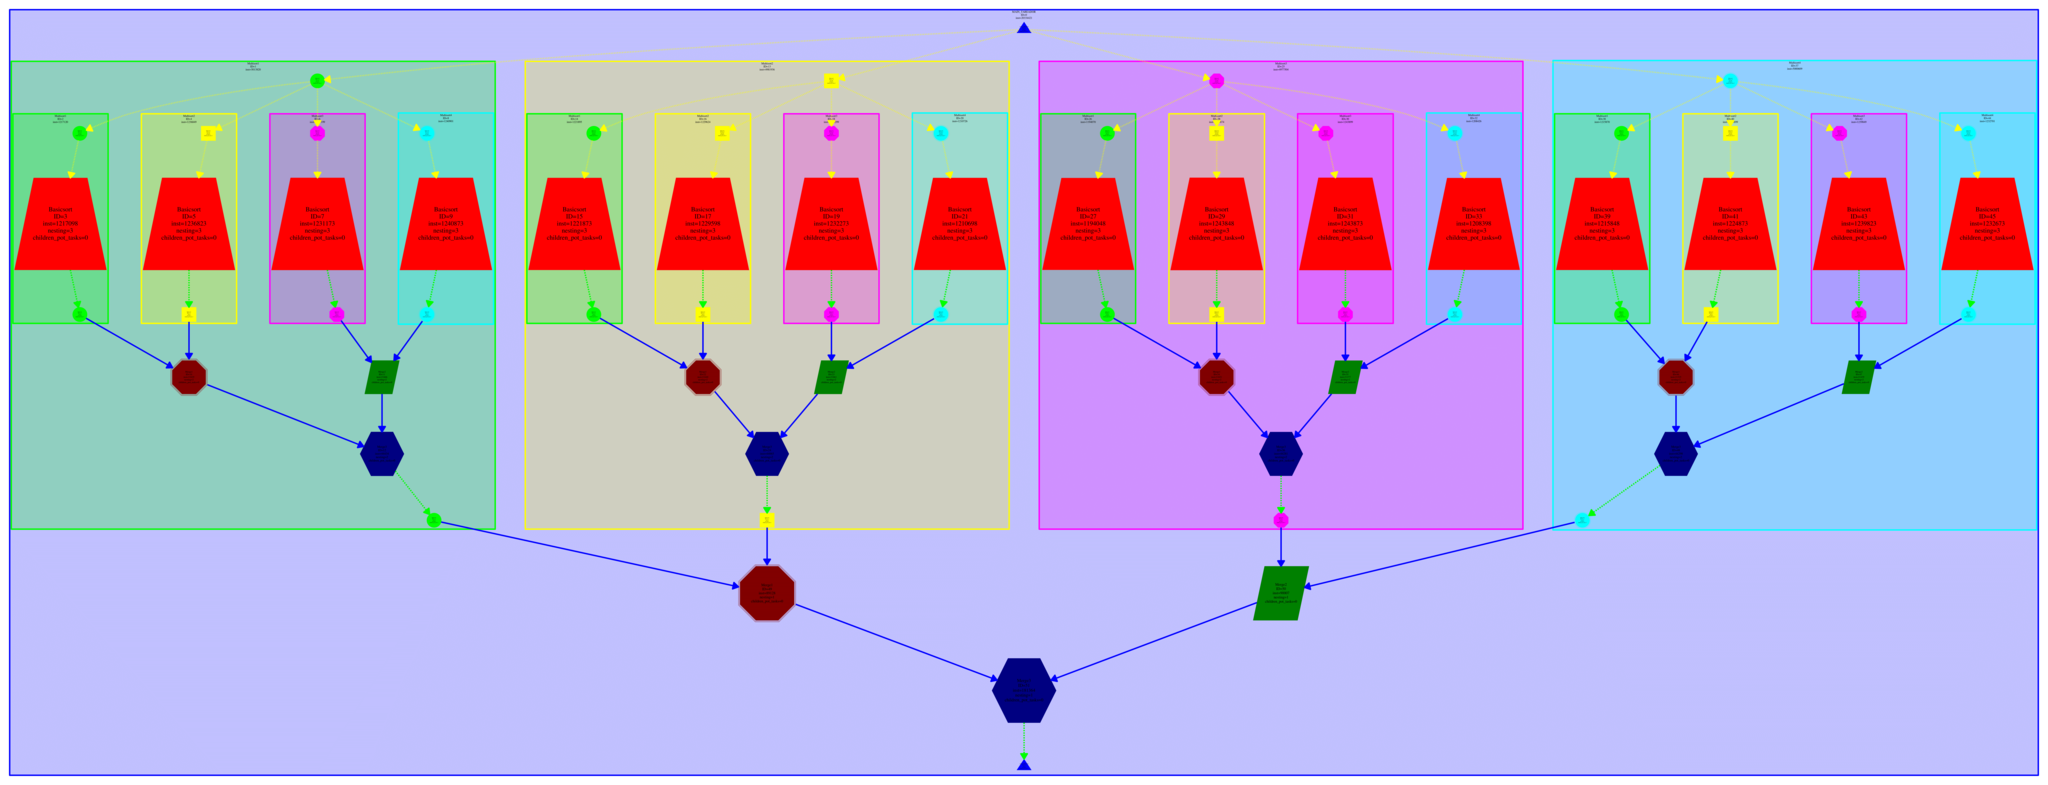
\includegraphics[width=\textwidth]{images/dependency_graph}
\end{figure}
	
	\question{Write a table with the execution time and speed-up predicted by \textit{Tareador} (for 1, 2, 4, 8, 16, 32 and 64 processors) for the task decomposition specified with Tareador. Are the results close to the ideal case? Reason about your answer.}
	
	\begin{figure}[H]
		\centering
		\begin{minipage}[t]{0.49\textwidth}
			\begin{tikzpicture}
			\begin{semilogxaxis}[
					xmin = 0, xmax = 64,
					log ticks with fixed point,
					xtick={1,2,4,8,16,32,64},
					xlabel = Number of processors,
					ylabel = Time (ms),
                    domain = 1:64
				]
				\addplot table[x=P,y=T]{data/tareador_time.csv};
                \addplot [mark=none, dashed]{20000/x};
			\end{semilogxaxis}
			\end{tikzpicture}
			\caption{Time by the number of processors}
		\end{minipage}
		\hfill
		\begin{minipage}[t]{0.49\textwidth}
			\begin{tikzpicture}
				\begin{semilogxaxis}[
						xmin=0, xmax=64,
						log ticks with fixed point,
						xtick={1,2,4,8,16,32,64},
						xlabel = Number of processors,
						ylabel = Speedup,
                        domain=1:20
					]
					\addplot table[x=P,y=S]{data/tareador_time.csv};
                    \addplot [mark=none, dashed]{x};
				\end{semilogxaxis}
			\end{tikzpicture}
			\caption{Speedup by number of processors}
		\end{minipage}
	\end{figure}

    As the graphics show, the results are close to the ideal case in up to 16 processors. The reason tat the speed-up doesn't increase with 32 and 64 processors is the task granularity or, in other words, the size of the problem introduced doesn't allow more than 16 tasks in parallel. 
\end{questionenum}

\section{Parallelization and performance analysis with tasks}
\begin{questionenum}
	\question{Include the relevant portion of the codes that implement the two versions (\textit{Leaf} and \textit{Tree}), commenting whatever necessary.}
	
    \begin{lstlisting}[language=C, title=\texttt{multisort-omp-tree.c}]
void merge(long n, T left[n], T right[n], T result[n*2], long start, long length) {
    if (length < MIN_MERGE_SIZE*2L) {
        // Base case
        basicmerge(n, left, right, result, start, length);
    } else {
        // Recursive decomposition
        #pragma omp task
        merge(n, left, right, result, start, length/2);
        #pragma omp task
        merge(n, left, right, result, start + length/2, length/2);
    }
}
    
void multisort(long n, T data[n], T tmp[n]) {
    if (n >= MIN_SORT_SIZE*4L) {
        // Recursive decomposition
        #pragma omp task
        multisort(n/4L, &data[0], &tmp[0]);
        #pragma omp task
        multisort(n/4L, &data[n/4L], &tmp[n/4L]);
        #pragma omp task
        multisort(n/4L, &data[n/2L], &tmp[n/2L]);
        #pragma omp task
        multisort(n/4L, &data[3L*n/4L], &tmp[3L*n/4L]);
        #pragma omp taskwait
        
        // Start a group of tasks to merge data
        #pragma omp taskgroup
        {
            #pragma omp task
            merge(n/4L, &data[0], &data[n/4L], &tmp[0], 0, n/2L);
            #pragma omp task
            merge(n/4L, &data[n/2L], &data[3L*n/4L], &tmp[n/2L], 0, n/2L);
        }
        
        // Start another group of tasks to merge the remaining two vectors, this group depends on
        // the previous taskgroup
        #pragma omp taskgroup
        {
            #pragma omp task
            merge(n/2L, &tmp[0], &tmp[n/2L], &data[0], 0, n);
        }
    } else {
        // Base case
        basicsort(n, data);
    }
}
    \end{lstlisting}
    
    
    \begin{lstlisting}[language=C, title=\texttt{multisort-omp-leaf.c}]
void merge(long n, T left[n], T right[n], T result[n*2], long start, long length) {
    if (length < MIN_MERGE_SIZE*2L) {
        // Base case for merge this is the only point to set a task
        #pragma omp task
        basicmerge(n, left, right, result, start, length);
    } else {
        // Recursive decomposition
        merge(n, left, right, result, start, length/2);
        merge(n, left, right, result, start + length/2, length/2);
    }
}

void multisort(long n, T data[n], T tmp[n]) {
    if (n >= MIN_SORT_SIZE*4L) {
        // Recursive decomposition
        multisort(n/4L, &data[0], &tmp[0]);
        multisort(n/4L, &data[n/4L], &tmp[n/4L]);
        multisort(n/4L, &data[n/2L], &tmp[n/2L]);
        multisort(n/4L, &data[3L*n/4L], &tmp[3L*n/4L]);
        
        #pragma omp taskwait
        merge(n/4L, &data[0], &data[n/4L], &tmp[0], 0, n/2L);
        merge(n/4L, &data[n/2L], &data[3L*n/4L], &tmp[n/2L], 0, n/2L);
        
        #pragma omp taskwait
        merge(n/2L, &tmp[0], &tmp[n/2L], &data[0], 0, n);
    } else {
        // Base case, in this implementation this is the only point to set the task
        #pragma omp task
        basicsort(n, data);
    }
}
    \end{lstlisting}
    
    \question{For the the Leaf and Tree strategies, include the speedup (strong scalability) plots that have been obtained for the different numbers of processors. Reason about the performance that is observed, including captures of Paraver windows to justify your explanations.}
    
    \begin{figure}[H]
        \centering
        \begin{minipage}[t]{0.49\textwidth}
            \begin{tikzpicture}
            \begin{axis}[
                    xmin=0,xmax=12,
                    xlabel=Number of processors,
                    ylabel=Time (ms),
                    domain=1:12
                ]
                \addplot table[x=P,y=T]{data/tree_time.csv};
                \addplot [mark=none, dashed]{6/x};
            \end{axis}
            \end{tikzpicture}
            \caption{Execution time of \texttt{multisort-omp-tree.c} by number of processors}
            \label{fig:tree_time}
        \end{minipage}
        \hfill
        \begin{minipage}[t]{0.49\textwidth}
            \begin{tikzpicture}
                \begin{axis}[
                        xmin=0,xmax=12,
                        xlabel=Number of processors,
                        ylabel=Speeup,
                        domain=1:12
                    ]
                    \addplot table[x=P,y=S]{data/tree_speedup.csv};
                    \addplot [mark=none, dashed]{x};
                \end{axis}
            \end{tikzpicture}
            \caption{Speedup of \texttt{multisort-omp-tree.c} by number of processors}
            \label{fig:tree_speedup}
        \end{minipage}
    \end{figure}


    \begin{figure}[H]
        \centering
        \begin{minipage}[t]{0.49\textwidth}
            \begin{tikzpicture}
                \begin{axis}[
                        xmin=0,xmax=12,
                        xlabel=Number of processors,
                        ylabel=Time (ms),
                        domain=1:12
                    ]
                    \addplot table[x=P,y=T]{data/leaf_time.csv};
                    \addplot [mark=none, dashed]{6/x};
                \end{axis}
            \end{tikzpicture}
            \caption{Execution time of \texttt{multisort-omp-leaf.c} by number of processors}
            \label{fig:leaf_time}
        \end{minipage}
        \hfill
        \begin{minipage}[t]{0.49\textwidth}
            \begin{tikzpicture}
                \begin{axis}[
                        xmin=0,xmax=12,
                        xlabel=Number of processors,
                        ylabel=Speedup,
                        domain=0:12
                    ]
                    \addplot table[x=P,y=S]{data/leaf_speedup.csv};
                    \addplot [mark=none, dashed]{x};
                \end{axis}
            \end{tikzpicture}
            \caption{Speedup of \texttt{multisort-omp-leaf.c} by number of processors}
            \label{fig:leaf_speedup}
        \end{minipage}
    \end{figure}
    
    Comparing the \autoref{fig:tree_speedup} and the \autoref{fig:leaf_speedup} it can be seen that the speedup is higher in the \texttt{tree} implementation than in the \texttt{leaf} implementation for the same number of processors. This is because the \texttt{leaf} implementation only allows the parallelization once \texttt{tree} implementation allows each task to do its own recursion allowing a better distribution of resources.
    
	\question{Analyze the influence of the recursivity depth in the \textit{Tree} version, including the execution time plot, when changing the recursion depth and using 8 threads. Reason about the behavior observed. Is there an optimal value?}
    
    \begin{figure}[H]
        \centering
        \begin{minipage}[t]{0.49\textwidth}
            \begin{tikzpicture}
                \begin{semilogxaxis}[
                        xmin=0,xmax=4096,
                        log ticks with fixed point,
                        xtick={1,2,4,8,16,32,64,128,256,512,1024,2048,4096},
                        xticklabels={1,2,4,8,16,32,64,128,256,512,1024,2048,4096},
                        x tick label style={yshift=-0.5ex,rotate=45, anchor=east},
                        xlabel = Recursion depth,
                        ylabel = Execution time
                    ]
                    \addplot table[x=D,y=T]{data/recursion_depth.csv};
                \end{semilogxaxis}
            \end{tikzpicture}
            \caption{Execution time by recursion depth}
        \end{minipage}
        \hfill
        \begin{minipage}[t]{0.49\textwidth}
            \begin{tikzpicture}
                \begin{semilogxaxis}[
                        xmin=0,xmax=4096,
                        log ticks with fixed point,
                        xtick={1,2,4,8,16,32,64,128,256,512,1024,2048,4096},
                        xticklabels={1,2,4,8,16,32,64,128,256,512,1024,2048,4096},
                        x tick label style={yshift=-0.5ex,rotate=45, anchor=east},
                        xlabel = Recursion depth,
                        ylabel = Seedup
                    ]
                    \addplot table[x=D,y=S]{data/recursion_depth.csv};
                \end{semilogxaxis}
            \end{tikzpicture}
            \caption{Speedup by recursion depth}
        \end{minipage}
    \end{figure}

    The optimal value is 256 of recursion depth. It obtains a good equilibrium between the execution time and the overhead introduced. A bigger number would make the speedup to be reduced and a smaller one would introduce more overhead.
\end{questionenum}



\section{Parallelization and performance analysis with dependent tasks}
\begin{questionenum}
	\question{Include the relevant portion of the code that implements the \textit{Tree} version with task dependencies, commenting whatever necessary.}
    
    This code allows for two possible implementations, one using only a \texttt{taskwait} solution and the other using both \texttt{taskwait} and \texttt{taskgroup}.
    
    \begin{lstlisting}[language=C, title=\texttt{multisort-omp-tree-dep-taskwait.c}]
// Solution using only taskwait

void merge(long n, T left[n], T right[n], T result[n*2], long start, long length) {
    if (length < MIN_MERGE_SIZE*2L) {
        // Base case
        basicmerge(n, left, right, result, start, length);
    } else {
        // Recursive decomposition
        #pragma omp task
        merge(n, left, right, result, start, length/2);
        #pragma omp task
        merge(n, left, right, result, start + length/2, length/2);
        
        // Wait for the same level tasks to finish
        #pragma omp taskwait
    }
}

void multisort(long n, T data[n], T tmp[n]) {
    if (n >= MIN_SORT_SIZE*4L) {
        // Recursive decomposition
        #pragma omp task depend(out: data[0])
        multisort(n/4L, &data[0], &tmp[0]);
        #pragma omp task depend(out: data[n/4L])
        multisort(n/4L, &data[n/4L], &tmp[n/4L]);
        #pragma omp task depend(out: data[n/2L])
        multisort(n/4L, &data[n/2L], &tmp[n/2L]);
        #pragma omp task depend(out: data[3L*n/4L])
        multisort(n/4L, &data[3L*n/4L], &tmp[3L*n/4L]);
        
        #pragma omp task depend(in: data[0], data[n/4L]) depend(out: tmp[0])
        merge(n/4L, &data[0], &data[n/4L], &tmp[0], 0, n/2L);
        #pragma omp task depend(in: data[n/2L], data[3L*n/4L]) depend(out: tmp[n/2L])
        merge(n/4L, &data[n/2L], &data[3L*n/4L], &tmp[n/2L], 0, n/2L);
        #pragma omp task depend(in: tmp[0], tmp[n/2L])
        merge(n/2L, &tmp[0], &tmp[n/2L], &data[0], 0, n);
        
        // Wait for all the same level tasks to finish
        #pragma omp taskwait
    } else {
        // Base case
        basicsort(n, data);
    }
}

    \end{lstlisting}
    
    \begin{lstlisting}[language=C, title=\texttt{multisort-omp-tree-dep-taskgroup.c}]
// Solution using both taskwait and taskgroup
    
void merge(long n, T left[n], T right[n], T result[n*2], long start, long length) {
    if (length < MIN_MERGE_SIZE*2L) {
        // Base case
        basicmerge(n, left, right, result, start, length);
    } else {
        // Recursive decomposition
        #pragma omp task
        merge(n, left, right, result, start, length/2);
        #pragma omp task
        merge(n, left, right, result, start + length/2, length/2);
    }
}

void multisort(long n, T data[n], T tmp[n]) {
    if (n >= MIN_SORT_SIZE*4L) {
        // Recursive decomposition
        #pragma omp task depend(out: data[0])
        multisort(n/4L, &data[0], &tmp[0]);
        #pragma omp task depend(out: data[n/4L])
        multisort(n/4L, &data[n/4L], &tmp[n/4L]);
        #pragma omp task depend(out: data[n/2L])
        multisort(n/4L, &data[n/2L], &tmp[n/2L]);
        #pragma omp task depend(out: data[3L*n/4L])
        multisort(n/4L, &data[3L*n/4L], &tmp[3L*n/4L]);
        
        #pragma omp task depend(in: data[0], data[n/4L]) depend(out: tmp[0])
        #pragma omp taskgroup // Wait all the tasks to finish
        {
            merge(n/4L, &data[0], &data[n/4L], &tmp[0], 0, n/2L);
        }
        #pragma omp task depend(in: data[n/2L], data[3L*n/4L]) depend(out: tmp[n/2L])
        #pragma omp taskgroup // Wait all the tasks to finish
        {
            merge(n/4L, &data[n/2L], &data[3L*n/4L], &tmp[n/2L], 0, n/2L);
        }
        #pragma omp task depend(in: tmp[0], tmp[n/2L])
        #pragma omp taskgroup // Wait all the tasks to finish
        {
            merge(n/2L, &tmp[0], &tmp[n/2L], &data[0], 0, n);
        }
        // Wait all the same level tasks to finish
        #pragma omp taskwait
    } else {
        // Base case
        basicsort(n, data);
    }
}
    \end{lstlisting}
	
	\question{Reason about the performance that is observed, including the speedup plots that have been obtained different numbers of processors and with captures of Paraver windows to justify your reasoning.}
    
    \begin{figure}[H]
        \centering
        \begin{tikzpicture}
            \begin{axis}[
                    width=0.7\textwidth,height=0.5\textwidth,
                    xmin=0,xmax=12,
                    xlabel=Number of processors,
                    ylabel=Speedup,
                    legend pos = north west,
                    domain=0:12
                ]
                \addplot table[x=P,y=S]{data/dep_taskgroup.csv};
                \addplot table[x=P,y=S]{data/dep_taskwait.csv};
                \addplot [mark=none, dashed] {x};
                \legend{Taskgroup, Taskwait}
            \end{axis}
        \end{tikzpicture}
        \caption{Speedup of \texttt{multisort-omp-dep-taskgroup.c} and \texttt{multisort-omp-dep-taskwait.c} by number of processors}
        \label{fig:dep}
    \end{figure}
    
    \begin{figure}[H]
    	\centering
    	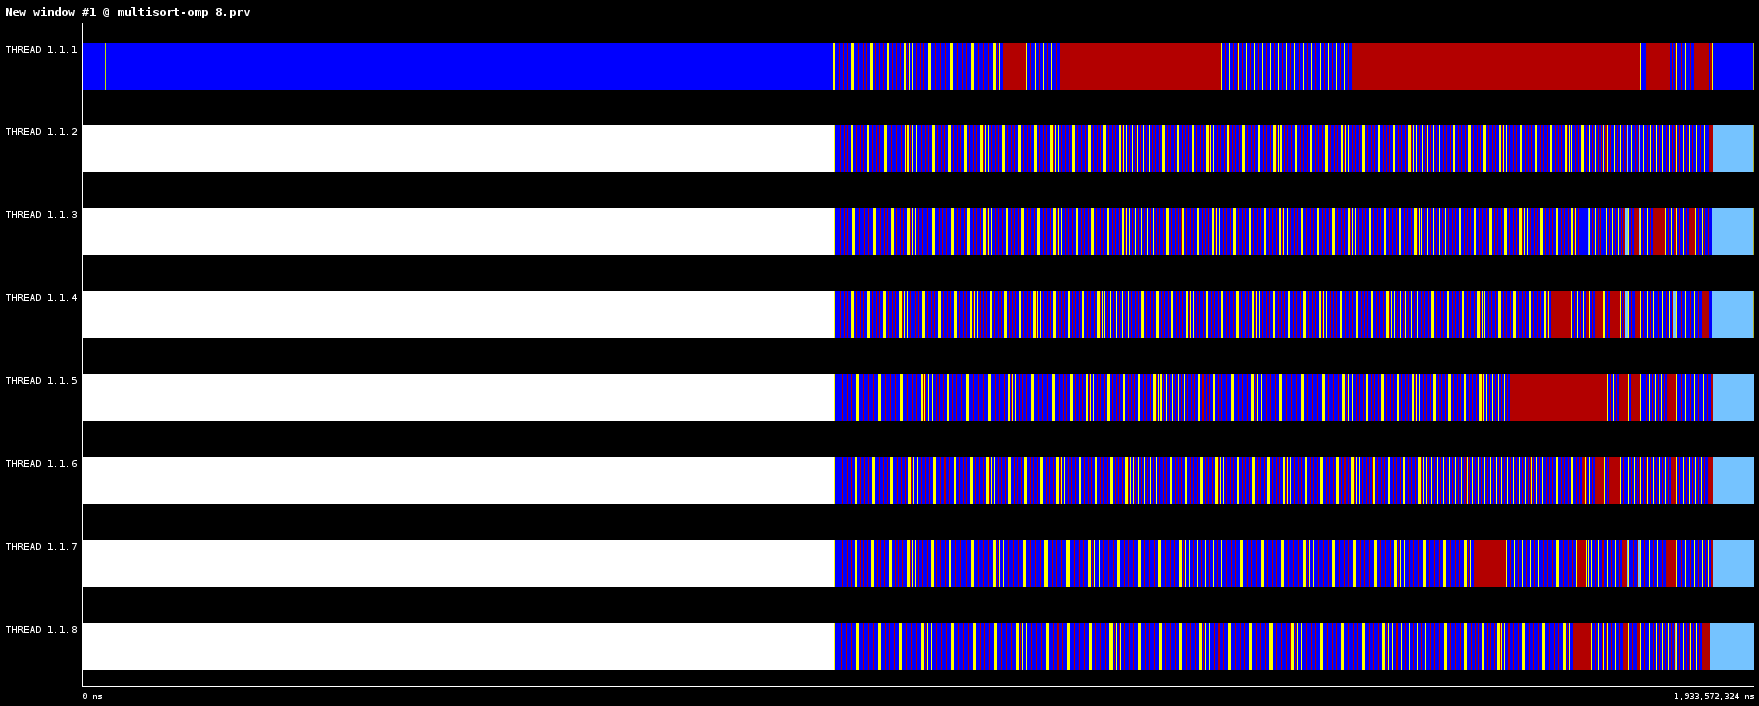
\includegraphics[width=\textwidth]{images/multisort-omp-paraver.png}
    	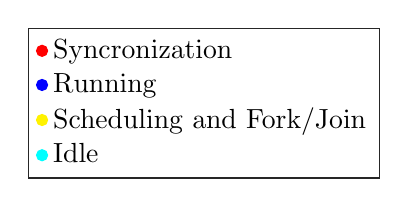
\begin{tikzpicture}
    		 \begin{axis}[
		    		 hide axis,
		    		 xmin = 10, xmax = 50, ymin = 0, ymax = 0.4,
		    		 legend style = { draw = white!15!black, legend cell align = left}
	    		 ]
	    		 \addlegendimage{only marks, red};
	    		 \addlegendentry{Syncronization};
	    		 \addlegendimage{only marks, blue};
	    		 \addlegendentry{Running};
	    		 \addlegendimage{only marks, yellow};
	    		 \addlegendentry{Scheduling and Fork/Join};
	    		 \addlegendimage{only marks, Cyan};
	    		 \addlegendentry{Idle};
    		 \end{axis}
    	\end{tikzpicture}
    \end{figure}
    
    The results show that the overhead starts increasing with more than 4 processors. As it can be seen in the \verb|Paraver| capture this is due to task synchronization.
    
    Comparing the two different versions of the \emph{Tree} version, there is a slightly increase of performance with \verb|taskgroup| as it was expected because there is less wait between the tasks.
\end{questionenum}

\section{Conclusion}
Thanks to the experiments that have been run, it can be seen that the \emph{Tree} implementation performs better than the \emph{Leaf} one. That is because the work of creating each task can be organized in different threads.

I has also been noticed a great improvement of performance when the task dependencies have been introduced. That reduced unnecessary waiting time of threads which leaded to smaller execution times.


\end{document}